\subsubsection[Jadex]{Jadex$^{\odot,\circ}$}\label{fun:apl_jadex}
This section presents Jadex, which is an agent framework focused on the development of goal-oriented agents following the belief-desire-intention model.
It aims at bringing middleware and reasoning-centred agent platforms together.
For that purpose, Jadex adds a rational reasoning engine to existing middleware.
The most commonly used middleware for Jadex is the \emph{Java Agent Development Framework} (short: JADE)~\cite{bellifemine_jade_2005}. %
Jadex integrates agent theories through object-oriented programming in Java and XML descriptions.
Therefore, no new language is introduced.
Jadex reuses already existing technologies instead.
JADE provides a communication infrastructure, platform services such as agent management and a set of development and debugging tools.
It enables the development and execution of peer-to-peer applications which are based on the agent paradigm (autonomous, proactive and social). % TODO We do not talk about this before. If you think, it is mandatory to mention agent paradigms here, you have to explain them. Also, build another sentence if needed but don't just add some buzzwords into brackets.
Autonomous and proactive mean, that an agent acts without human intervention or guidance.
Social here means that agents should work together to accomplish their goals.

Agents are identified by a unique name and provide a set of services.
They can register and modify their services and/or search for agents providing given services.
Additionally they are capable of controlling their life cycle and they can dynamically discover other agents and communicate with them.
% TODO @manuelmittler what does it mean to control its own lifecycle? -> activate/kill the agent
The communication happens by exchanging asynchronous messages via an \emph{agent communication language} (short: ACL).
Jadex complies with the standard given by the Foundation for Intelligent Physical Agents (FIPA).
FIPA \blockquote[\cite{FIPA}][.]{is an international organisation that is dedicated to promoting the industry of intelligent agents by openly developing specifications supporting interoperability among agents and agent-based applications}
A FIPA ACL message has a certain structure and contains five mandatory parameters.
The first is the type of the communicative act which tells the recipient how to react on the message.
Next, the participants in the communication, namely sender and receiver, are specified.
The third parameter contains the actual content of the message.
As a fourth parameter, there is the description of the content which denotes the language of the content and its encoding.
The last parameter is called control of conversation and contains, amongst other things, a conversation identifier.
Its purpose is to associate a message with a specific conversation and to chronologically sort it in said conversation.

\begin{figure}
	\centering
	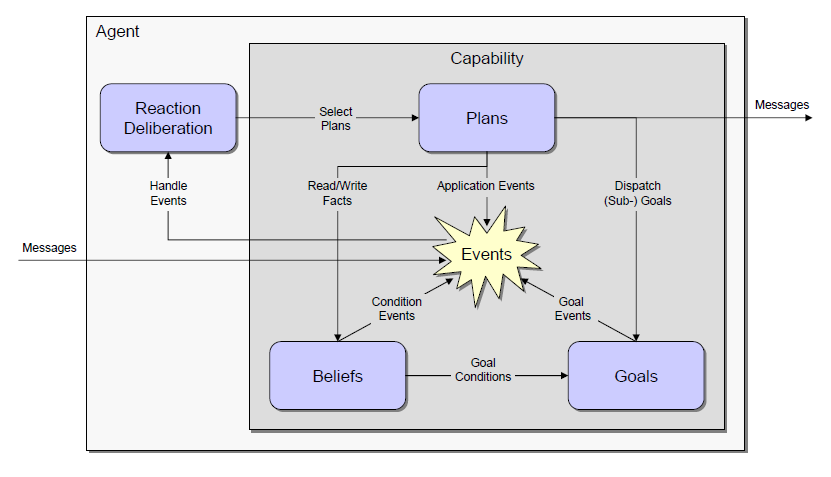
\includegraphics[width=300px]{images/Jadex_agent.png}
	\caption{Jadex abstract agent~\cite{pokahr_jadex_2005}}
	\label{fig:apl_jadex1}
\end{figure}
\autoref{fig:apl_jadex1} depicts an abstract view of a Jadex agent.
Every agent may receive messages which trigger internal events that can change his internal knowledge, plans or goals.
Interactions with the \enquote{outside}, like the environment or other agents, happens through the sending of messages. % TODO @manuelmittler I removed the quote as I did not find it to be necessary here. Am I correct that modifications in the environment are also done through messages? These modifications are nothing we have in our scenario but in many others, agents' actions effect the world they are active in.
In more detail, beliefs are single facts stored as Java objects which represent the knowledge of an agent.
They are stored as key-value pairs.
The advantage of storing information as facts is that the programmer has a central place for the knowledge and can query the agent's beliefs. % TODO @manuelmittler or do you mean that there is an advantage by storing them as Java Objects? -> yes
Monitoring of the beliefs is possible too.

Goals are momentary desires of an agent for which the agent engages into suitable actions until it considers the goal as being reached, unreachable, or not wanted any more.
Referring to~\cite{ActiveComponentsGoals}, Jadex distinguishes between four generic goal types.
A \emph{perform goal} is directly related to the execution of actions.
Therefore, the goal is considered to be reached when some actions have been executed, regardless of the outcome of these actions.
An \emph{achieve goal} is a goal in the traditional sense, which defines a desired world state without specifying how to reach it.
Agents may try several different alternative plans, to achieve a goal of this type.
A \emph{query goal} is similar to an achieve goal, but the desired state is not a state of the (outside) world, but an internal state of the agent, regarding the availability of some information the agent wants to know about.
For goals of type \emph{maintain}, an agent keeps track of a desired state, and will continuously execute appropriate plans to re-establish this maintained state whenever needed.
In contrast to goals, events are by default dispatched to all interested plans but do not support any BDI-mechanism.
Therefore, the originator of an internal event is usually not interested in the effect the internal event may produce but only wants to inform some interested parties about some occurrence.
Plans represent the behavioural elements of an agent and are composed of a head and a body part.
The plan head specification is similar to other BDI systems and mainly specifies the circumstances under which a plan may be selected, e.g.\ by stating events or goals handled by the plan and preconditions for the execution of the plan.
Additionally, in the plan head a context condition can be stated that must be true for the plan to continue executing.
The plan body provides a predefined course of action, given in a procedural language.
This course of action is to be executed by the agent, when the plan is selected for execution, and may contain actions provided by the system API, such as sending messages, manipulating beliefs, or creating sub-goals (cf.~\cite{braubach_jadex_2004})

Jadex is not based on a new agent programming language but chooses a hybrid approach instead.
It distinguishes explicitly between the language used for static agent type specification as shown in \autoref{fig:jadex_active_components} and the language for defining the dynamic agent behaviour.
An agent in Jadex consists of two components: An \emph{agent definition file} (short: ADF) for the specification of beliefs, goals, and plans as well as their initial values and on the other hand procedural plan code.
\begin{figure}
	\centering
	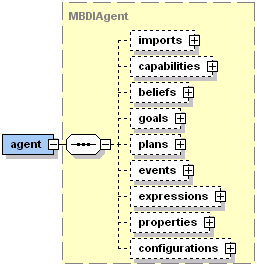
\includegraphics[height=200px]{images/jadexagentadf.png}
  \caption{Jadex top level ADF elements \cite{ActiveComponents}}
	\label{fig:jadex_active_components}
\end{figure}
The procedural part of plans (the plan bodies) are realised in an ordinary programming language (Java) and have access to the BDI facilities of an agent through an application interface (API).
The plan body is a standard Java class that extends a predefined Jadex framework class.
It must at least implement the abstract \texttt{body()} method which is invoked after plan instantiation.
To stick to the previously used coffee example, the Java code for this Plan has to be implemented in the corresponding method.
The body of the methods in \autoref{lst:jadex_java} is intentionally left blank because the focus of this section is set on Jadex instead of ordinary Java code.
\begin{lstlisting}[caption={Jadex Java class.}, label=lst:jadex_java]
public class ServeCoffeePlanB1 extends Plan {
   // Plan attributes.

   public ServeCoffeePlan() {
       // Java code for plan "ServeCoffeePlan".
   }

   public void body() {
       // Initialisation code.
   }
}
\end{lstlisting}
The plan body is associated to a plan head in the ADF.
This means that in the plan head, several properties of the plan can be specified, e.g.\ the circumstances under which it is activated and its importance in relation to other plans as shwon in \autoref{lst:jadex_xml}.
\begin{lstlisting}[caption={Jadex XML file.}, label=lst:jadex_xml]
<agent xmlns="http://jadex.sourceforge.net/jadex-bdi"
 xmlns:xsi="http://www.w3.org/2001/XMLSchema-instance"
 xsi:schemaLocation="http://jadex.sourceforge.net/jadex-bdi
            http://jadex.sourceforge.net/jadex-bdi-2.0.xsd"
 name="CoffeeAgent">

 <plans>
   <plan name="serve">
     <body class="ServeCoffeePlan"/>
     <waitqueue>
       <messageevent ref="request_serving"/>
     </waitqueue>
   </plan>
 </plans>

 <events>
   <messageevent name="request_serving"
                 direction="receive" type="fipa">
     <parameter name="performative" class="String"
                direction="fixed">
       <value>jadex.bridge.fipa.SFipa.REQUEST</value>
     </parameter>
   </messageevent>
 </events>

 <properties>
   <property name="debugging">false</property>
 </properties>

 <configurations>
   <configuration name="default">
     <plans>
       <initialplan ref="serve"/>
     </plans>
   </configuration>
 </configurations>
</agent>
\end{lstlisting}
There are two types of plans in Jadex.
A \emph{service plan} and a \emph{passive plan}.
The service plan, as the name indicates, is an instance of a plan which waits for service requests.
Therefore, a service plan can set up its private event wait queue and receive events for later processing, even when it is working at the moment.
In contrast to that, a passive plan is only running when it has a task to achieve.
For this kind of plan the triggering event and goals must be specified in the agent definition file to let the agent know which kinds of events this plan can handle.
When an agent receives an event, the BDI reasoning engine builds up the so-called applicable plan list which contains all plans that can handle the current event or goal.
The candidates are selected and instantiated for execution.

The execution model for Jadex looks like it is shown in \autoref{fig:jadex_execution_model} following:
\begin{figure}
	\centering
	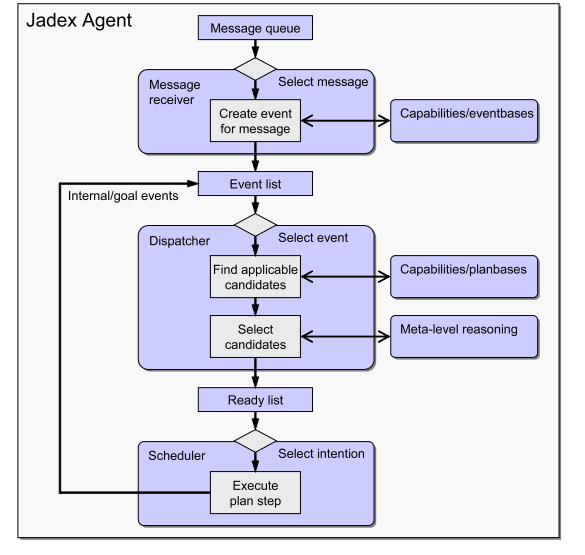
\includegraphics[width=300px]{images/Jadex_execution_model.png}
	\caption{Jadex execution model \cite{pokahr_jadex_2005}}
	\label{fig:jadex_execution_model}
\end{figure}

When an agent receives a message, it is placed on a message queue.
In the next step, the message has to be assigned to a capability which can handle the message.
A suitable capability is found by matching the message against the event templates defined in the event base of each capability.
The best matching template is then used to create an appropriate event in the scope of the capability.
After that the created event is subsequently added to the agent's global event list.
The dispatcher is responsible for selecting applicable plans for the events from the event list.
After plans have been selected, they are placed in the ready list, waiting for execution.
The execution of plans is performed by a scheduler, which selects plans from the ready list~\cite{pokahr_jadex_2005}.

In summary, Jadex is a powerful framework that supports easy agent construction with XML-based agent description and procedural plans in Java.
Additionally, it offers tool support for debugging during development.
For example, it comes with a graphical BDI viewer that allows observing and modifying the internal state of an agent and a logger agent that collects log-outputs of any agent.
